\documentclass[12pt, letterpaper]{article}
\usepackage[utf8]{inputenc}
 \usepackage[letterpaper, margin=0.8in]{geometry}
 \usepackage{amssymb}
\usepackage{amsmath}
 \usepackage{enumitem}
\usepackage {listings}
\usepackage{pgfplots}
\usepgfplotslibrary{external}
\usepackage{graphicx}

\title{CS425 Project 3(Report)\\k-Nearest-Neighbors and Decision Trees}
\author{Ksenia Burova}
\date{November \(6^{th}\), 2017}

\begin{document}
\maketitle

{\noindent {\bf Abstract:} Th In this project, we were given data file with different attributes that correspond to breast cancer diagnosis. The goal of the project was to run both, kNN and Decision Trees algorithms, to see how well they perform in predicting a tumor being benign or malignant. In machine learning, k-Nearest-Neighbors (kNN) algorithm is one of the nonparametric estimation methods, and in nonparametric methods we assume that similar data inputs have similar data outputs, and we go from there. Decision Trees algorithm belongs to the family of supervised learning classification algorithms, in which the target variable has some numerical values, and at each step of the algorithm we decide how to split data depending on one of those values. After implementing both algorithms we had to measure performance. There were several performance metrics to be used to analyze results. Some of those metrics were displayed in plots. \\
For {\bf  extra credit }, we had to reduce given data to some number of PCs, as we did in Project 2, and to perform Decision Trees part on new sets of data. }

\begin{enumerate}[label=\Roman*.]
	
	{\bf \item Project Data.} \\
	
	 In this project, we were given a file {\it breast-cancer-wisconsin.data} which had 11 attributes:
	 \begin{enumerate}[label=\arabic*.]
	 	\item Sample code number: id number
		\item Uniformity of cell size: 1 - 10
		\item Uniformity of Cell Shape: 1 - 10
		\item Marginal Adhesion: 1 - 10
		\item Single Epithelial Cell Size: 1 - 10
		\item Bare Nuclei: 1 - 10
		\item Bland Chromatin: 1 - 10
		\item Normal Nucleoli: 1 - 10
		\item Mitoses: 1 - 10
		\item Class: (2 for benign, 4 for malignant)
	\end{enumerate}
	
	I removed a column with {\bf id number}  since it is not relevant in predicting tumor type. There were also some data with missing values. My choice was not to predict those values, instead, I excluded that data from the data set. I decided to use such method to avoid incorrect prediction that may influence experiment results. \\
	
	I've placed all continuous values for this data into multidimensional array called {\bf dataFeatures}, and kept classes in one-dimensional array called {\bf dataLabels} for simplicity of implementation. \\
	During experiments, data was split into 3 sets: training, validation and testing. First I've split the whole data into training and testing data sets with 70/30 proportion rule. Then training data was divided into training and validation parts with 70/30 proportion rule as well for cross validation purposes. \\
	
	{\bf \item Tools and Program.}\\
	
	I've used {\bf python} programming language, {\bf numpy} library for arithmetic, {\bf sklearn} library for splitting my data into training, validation and testing datasets, and {\bf matplotlib} library to built plots for this project. I have a program named {\bf knn-dt.py} , that includes implementation of both parts of the project. I've split each algorithm into several functions for efficiency, and in the very end of my program I do main calls to run experiments and build plots.\\
	
	{\bf \item Performance metrics.}\\
	
	To evaluate performance of  classification algorithms, we have to compare correct classifications with our classifications on evaluation data sets after algorithm is run. We are going to calculate and look at the following values: 
	\begin{itemize}
		\item Confusion Matrix \\
		
		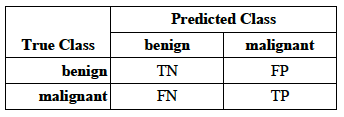
\includegraphics[scale=0.7]{../images/1.png} \\
		where TP = \# true positives, TN = \# true negatives, FP = \# false positives, FN = \# false negatives.\\
		
		\item Accuracy = (TN + TP) / (TN + TP + FN + FP)\\
		{\bf Accuracy} tells us what percent of data was classified correctly. \\
		\item TPR (true positive rate, recall, or sensitivity) = TP / (TP + FN)\\
		{\bf Sensitivity} shows us rate at which true positives are not missed/overlooked \\
		\item PPV (positive predictive value or precision) = TP / (TP + FP)\\
		{\bf Precision} is basically a fraction of relevant positive data from all the positive data we have, meaning have many of those diagnosed with bad cancer really have it. \\ 
		\item TNR (true negative rate or specificity) = TN / (TN + FP)\\
		{\bf Specificity} is a rate that shows how well we can distinguish data that is truly negative, meaning that people have good tumor.\\
		\item F Score = PPV * TPR / (PPV + TPR)\\
		{\bf F score} is a harmonic average of precision and sensitivity, it is basically used if we can't decide with of 2 metrics to use for performance measurements. \\
	\end{itemize}
	
	{\bf \item Part 1. k-Nearest-Neighbors. }\\
	
	kNN algorithm, as all nonparametric algorithms, is composed of finding the similar instances from the training set using one of distance measures and interpolating from them to find the right output. Distance measures may differ but in our experiment we are going to use Euclidian distance between two multidimensional data points:\\
	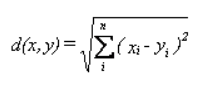
\includegraphics[scale=0.7]{../images/d1.png} 
	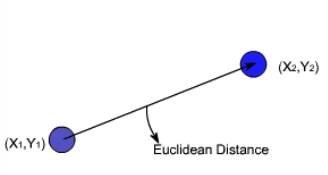
\includegraphics[scale=0.5]{../images/d2.png} 
	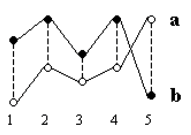
\includegraphics[scale=0.7]{../images/d3.png} \\
	
	\begin{enumerate}[label=\arabic*.]

	\item {\it Calculating Neighborhood. }\\
	The first part of the algorithm after splitting datasets, is to calculate distances for each evaluation(validation or testing) data point and all data points in training set. After that we choose k data points from training set which become k nearest neighbors, obviously. So, our neighborhood for each evaluation data point consists of training data points that are the closest distance-wise. We've used different values of k in this project to compare performance and determine the best ones. The values were following: 2, 3, 4, 5, 6, 7, 8, 16, 32.\\
	
	\item {\it Classification. }\\
	When neighborhood is known for each  evaluation data point, we can classify those data points. What we do is counting votes of each neighbor for class and choose class with the maximum number of votes. For example, if we have three neighbors and two of them are benign and one is malignant, that means that two neighbors vote for class '2', and one votes for class '4'. Since we have more votes for class '2', our evaluation data point will be classified as benign. There are ties possible, in this case I always make evaluation data point to be classified as malignant. Not only it's the one of the most common ties resolutions, in my mind, it makes sense. If we can't be really positive on tumor being good it's better to mark it as bad. \\
	
	\item {\it Performance. }\\
	After we are done with the major part of algorithm, we have to run it for multiple k values to determine the most optimal one. Before we run kNN for all values, we split training set into training and validation parts. We predict classification for validation set and compare them with real values. For performance metrics, we use confusion matrix that records number of true-positive, true-negative, false-positive and false-negative values. Using metrics from confusion matrix, we calculate prediction accuracy and other relevant measurements of performance. \\
	
	Results for k = 2, 3, 4, 5, 6, 7, 8, 16, 32 look as following: \\
	\begin{center}
	 	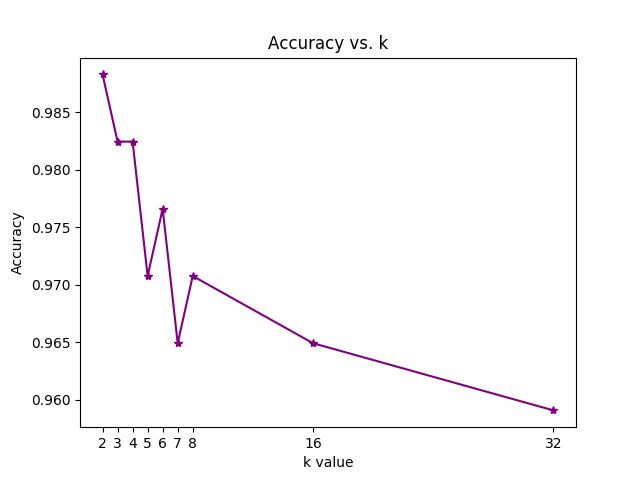
\includegraphics[scale=0.7]{../images/accuracy.png} 
	\end{center}
	 As we can see, in my experiment, using 2 neighbors gives us the most accurate results, almost 0.99 correct prediction. Of course this value depends on how you split data set. I used seed= 26 for random number generator to split data into sets. \\
	 Having 3 and 4 neighbors also gives us pretty good accuracy, and accuracy drops if we use more neighbors. \\
	 
	 Let's look at other parameters: \\
	\end{enumerate}
	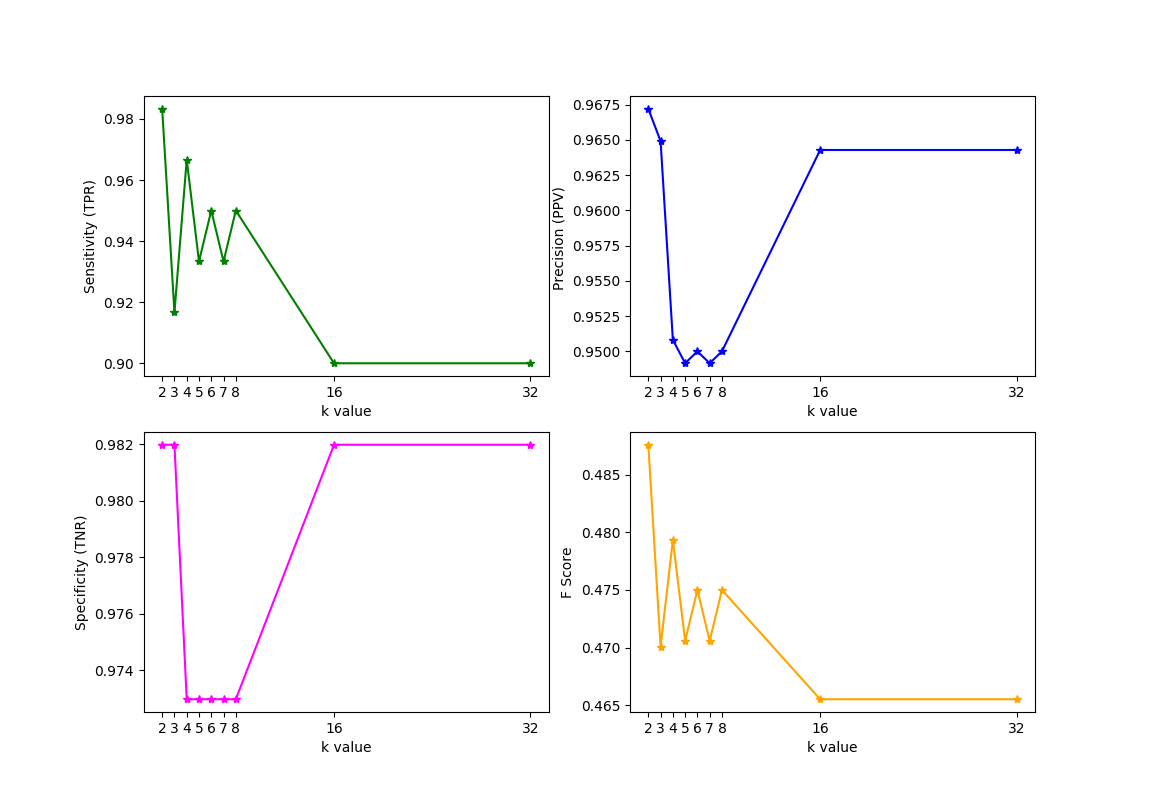
\includegraphics[scale=0.65]{../images/metrics.png} 
	It is obvious that Sensitivity, precision and F Score have identical pattern, and specificity is constant in my case. So I would say that yes, having 2 neighbors gives me the best classification performance. \\
	
	After I ran kNN algorithm on my testing data set I received following values:
	\begin{verbatim}		
		Confusion matrix =  [[116, 4], [1, 50]] 
		Accuracy = 0.9707
		Sensitivity = 0.9803
		Precision = 0.9259
		Specificity = 0.9666
		F Score = 0.4761
	\end{verbatim}
	
	So, we have results slightly lower than on validation set, but accuracy of 0.97 is still pretty high, so we can call our prediction to be completed successfully. Let's look at how Decision Trees algorithm performed next.
	
	{\bf \item Part 2. Decision Trees. }\\
	A decision tree is a hierarchical model for supervised learning where locality of a datapoint among classes is identified in a sequence of recursive splits in a smaller number of steps. Decision tree is composed of internal nodes and leafs, where internal nodes hold an attribute upon with decision is made when going down the tree. Leaf nodes contain a class identifier. In some cases it is possible that one leaf can hold more than two class values. This is how tree would look when classifying data:\\
	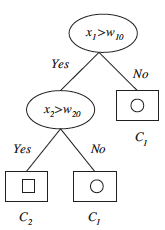
\includegraphics[scale=0.9]{../images/2.png} \\
	So, as you can see, at each step we look at some attribute and decide if our datapoint has to go to the right or to the left to make next decision. \\
	In decision tree for classification, the goodness of a split is quantified by an impurity measure. A split is pure if after the split, for all branches, all the instances choosing a branch belong to the same class. There are several impurity measurements can be used in classification: \\
	\begin{enumerate}
		\item Entropy\\
		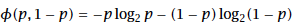
\includegraphics[scale=0.7]{../images/4.png} \\
		\item Gini Index \\
		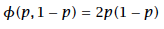
\includegraphics[scale=0.7]{../images/5.png} \\
		\item Misclassification Error\\
		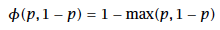
\includegraphics[scale=0.7]{../images/6.png} \\
	\end{enumerate}
	All these measures are very similar. In general, If node m is not pure, then the instances should be split to decrease impurity. We check all attributes to see which one could give us the best split, or in other words, the one that minimizes impurity. \\
	
	Let's dive into results.\\
	
	\begin{enumerate}[label=\arabic*.]
		\item {\it Algorithm. }\\
		
		The algorithm for my implementation was taken from from the book with some tweaks into it to make it work with the project requirements.\\
		
		 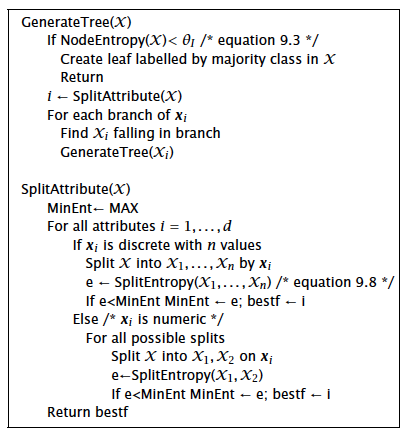
\includegraphics[scale=0.7]{../images/7.png} \\
		 So , instead of using just entropy, I can pass all three impurity functions, I also terminate depending on a tree depth or threshold that user passes.\\
		 
		\item {\it Termination By Depth. }\\
		
		In my first experiment, I was terminating from the tree when maximum length of the tree was reached or when we couldn't split no more. As was suggested in a write up, I used values k = 2 ,3, 4, 5, 6, 7, 8, 16, 32. The accuracy results for that run for all 3 impurity functions look as following:\\
		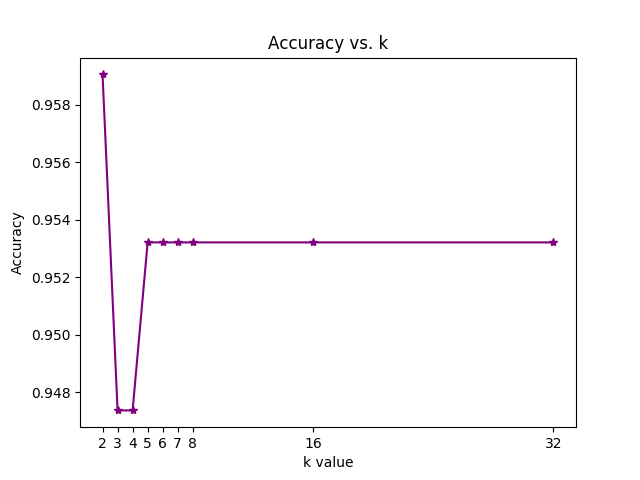
\includegraphics[scale=0.7]{../images/accuracy_validation_DT_Depth_error_0.png} \\ 
		
		Also I have to mention, that k starts with 0 in my code, so technically those values are k+1. \\
		I really think that k = 2 being the best seems kind of weird, but it's value of accuracy is almost the same as for larger numbers for depths. In general, accuracy becomes more consistent when tree is deeper. For straight line that we observe, depth = 6. With my dataset , that's how deep my tree can possibly go. When I look at the result for testing data with k = 2, or depth = 3, it is pretty low: \\
		\begin{verbatim}		
		Confusion matrix =  [[112, 8], [4, 47]] 
		Accuracy = 0.9298
		Sensitivity = 0.9215
		Precision = 0.8545
		Specificity = 0.9333 
		F Score = 0.4433
		\end{verbatim}
		
		So, something went wrong. \\
		
		\item {\it Termination By Threshold. }\\
		
		Another way to stop constructing the tree, when a value of passed by user threshold is passed. I've ran several experiments for threshold values ranging from 0 to 0.5 as well and got following results, identical for all three functions as well: \\
		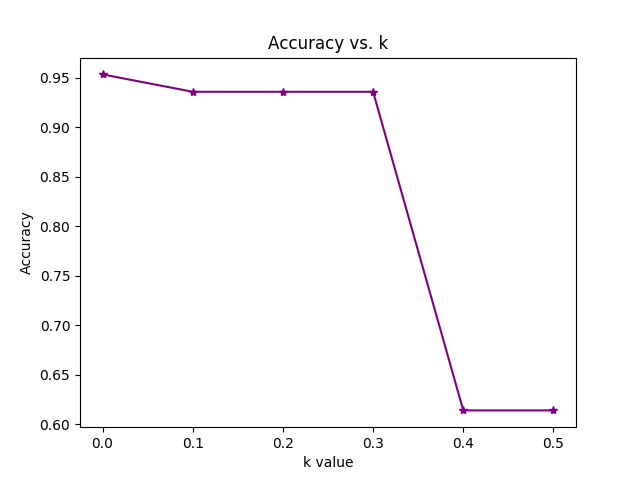
\includegraphics[scale=0.7]{../images/accuracy_validation_DT_Threshold_gini.png} \\ 
		In this case, it looks good to me. Basically, how impurity threshold works, If we pass too large entropy our data doesn't get split much and tree doesn't have a big depth and thus all leaf nodes are not very pure. With passing lower threshold value we expect nodes to have lower impurity and this way better classification capability. So, passing 0 for threshold gave us the best result. Tree depth for it is 6. Next 3 values have tree depth of 2, and obviously with too high threshold we never split first node, so depth = 1.  \\Let's look at testing data classification results: 
		\begin{verbatim}		
		Confusion matrix =  [[102, 3], [5, 61]] 
		Accuracy = 0.9532
		Sensitivity = 0.9242
		Precision = 0.9531
		Specificity = 0.9714
		F Score = 0.4692
		\end{verbatim}
		
		Accuracy is high enough to say that classification was successful. \\
		
		\item {\it PCAs. }\\ 
		
		In this project our data has 10 dimensions. It's hard to visualize it that way. So we are going to try to reduce number of dimensions. We also want to observe results of classification here.  So we are going to use PCA that we implemented in previous project and we'll try to reduce that to first 2, 4 and 6 components. I've showed that my software does both, tree termination by depth and by threshold, so in this experiment I will only display results when we terminate tree by threshold. \\
		
		There results of accuracy for all 3 impurity functions for values 2, 4 and 6 were the following: \\
		
		Entropy Impurity function: \\
		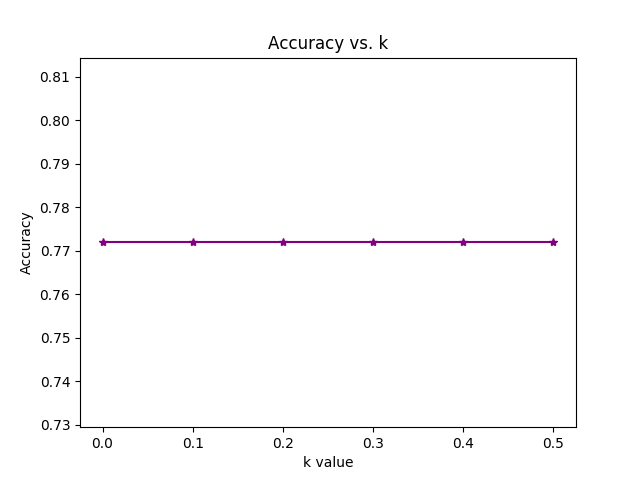
\includegraphics[scale=0.5]{../images/accuracy_validation_DT_Threshold_entropy_2.png} 
		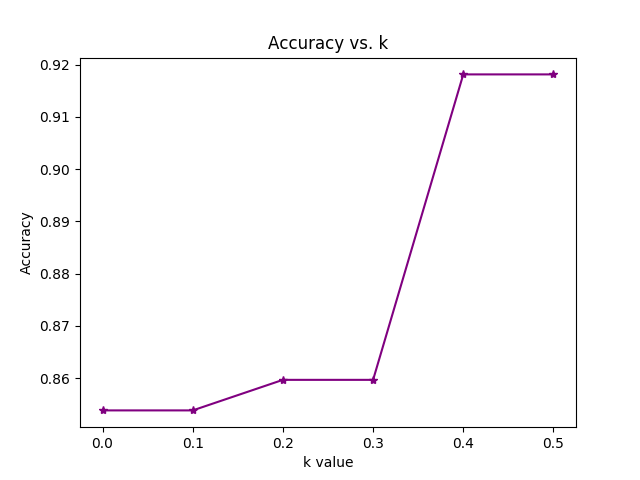
\includegraphics[scale=0.5]{../images/accuracy_validation_DT_Threshold_entropy_4.png} 
		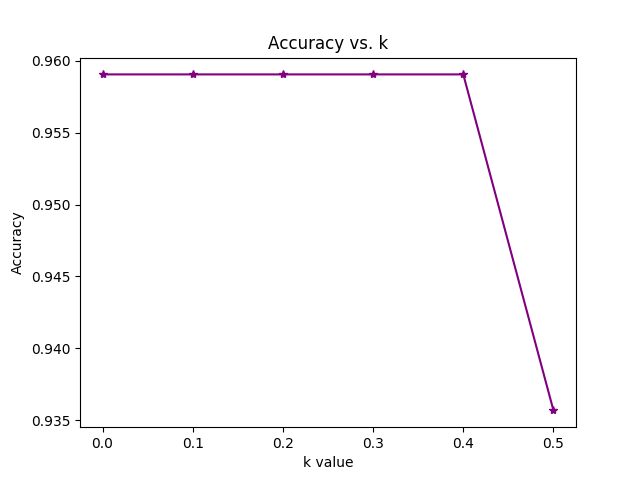
\includegraphics[scale=0.5]{../images/accuracy_validation_DT_Threshold_entropy_6.png} \\
		
		For PCs = 2, results are very consistent, for PCs = 4, results are unexpected, for PCs = 6 we have good results where accuracy is high with lower threshold values. It is also pretty consistent.\\
		
		Gini Impurity function: \\
		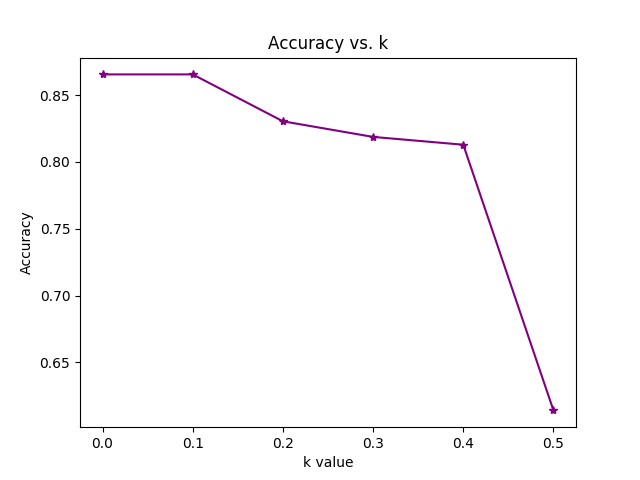
\includegraphics[scale=0.5]{../images/accuracy_validation_DT_Threshold_gini_2.png} 
		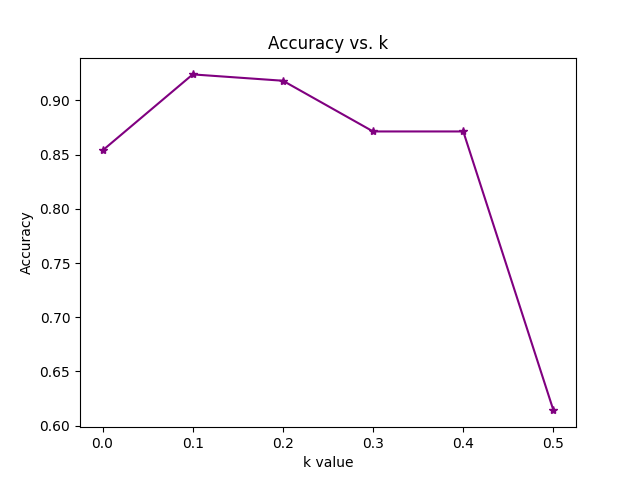
\includegraphics[scale=0.5]{../images/accuracy_validation_DT_Threshold_gini_4.png} 
		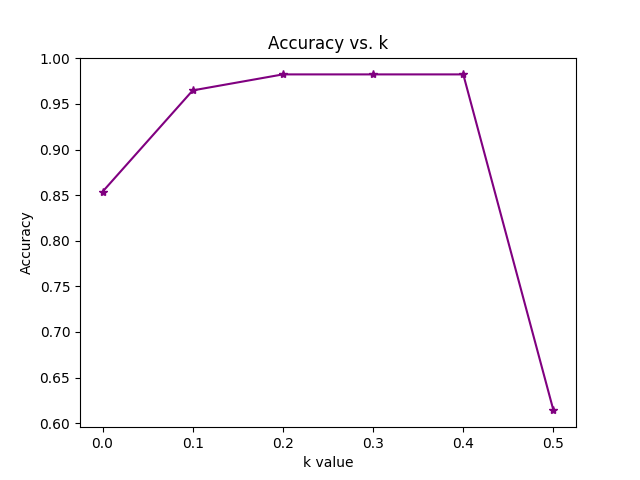
\includegraphics[scale=0.5]{../images/accuracy_validation_DT_Threshold_gini_6.png} \\
		
		With Gini function, all PCs values have similar results, but PCs = 2 seems to be the most consistent. It gives better accuracy for lower threshold. Bit PCS = 6 again reaches better accuracy at some point. \\
		
		Misclassification Error: \\
		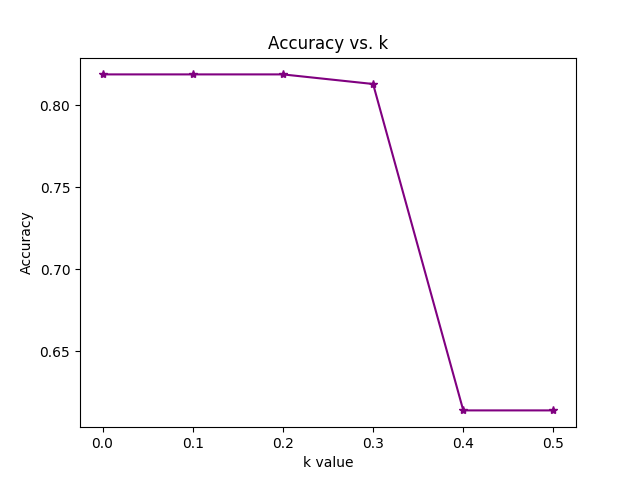
\includegraphics[scale=0.5]{../images/accuracy_validation_DT_Threshold_error_2.png} 
		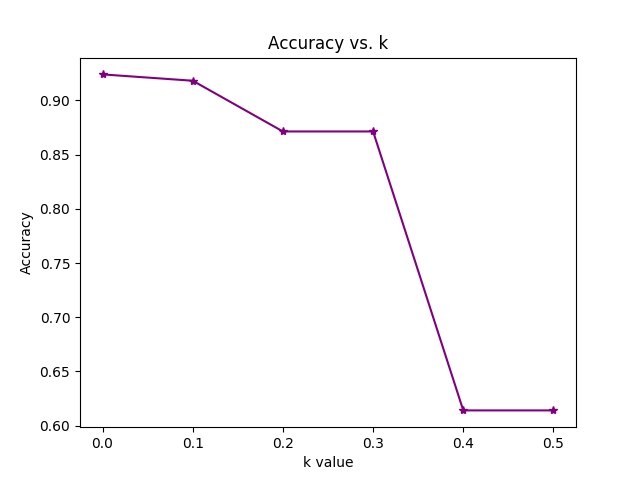
\includegraphics[scale=0.5]{../images/accuracy_validation_DT_Threshold_error_4.png} 
		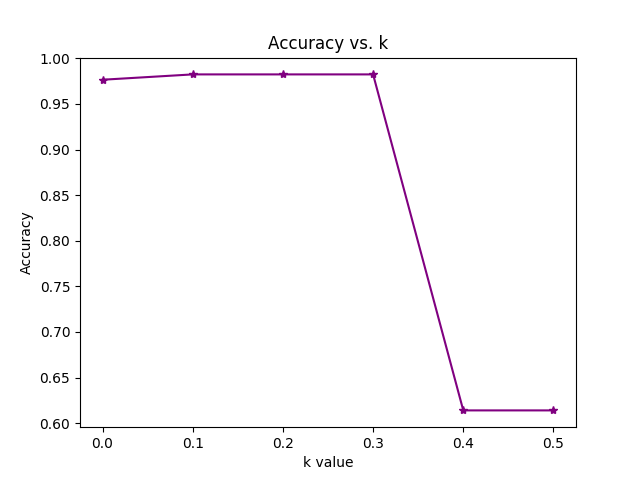
\includegraphics[scale=0.5]{../images/accuracy_validation_DT_Threshold_error_6.png} \\
		
		Misclassification Error function is the best here. Pattern is similar for all number of PCs, but PCs = 6 has higher accuracy again. \\
		
		I didn't try to plot 6 PCS cause it is somewhat hard. But I've tried to look at scatter plots for first 2 PCs for our trained data. Here is how we classified our data: \\
		
		There order of images is Entropy, Gini, Misclassification Error: \\
		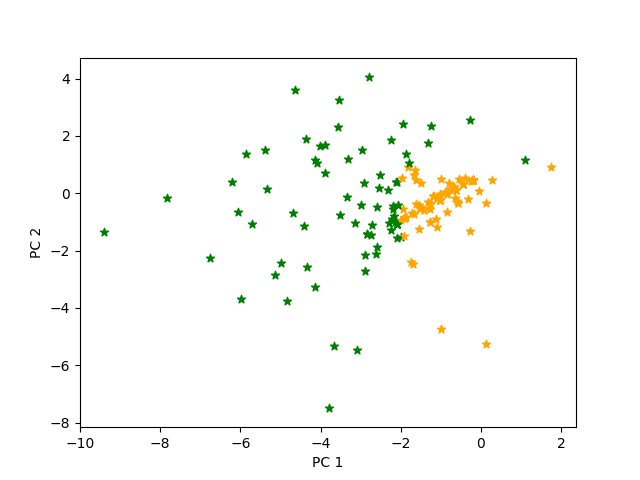
\includegraphics[scale=0.5]{../images/clusters_entropy_Depth_.png} 
		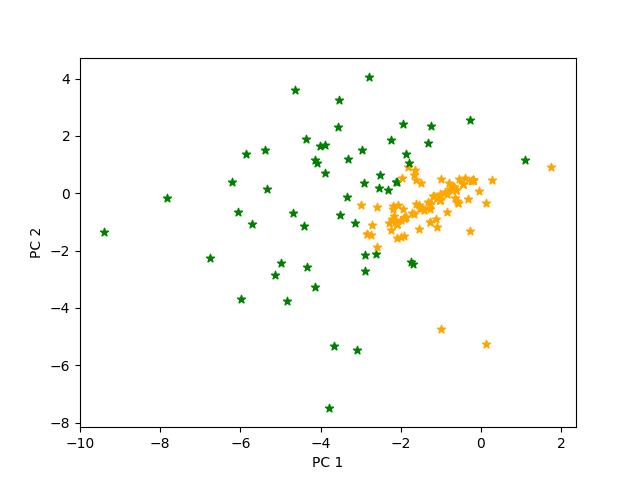
\includegraphics[scale=0.5]{../images/clusters_gini_Depth_.png} 
		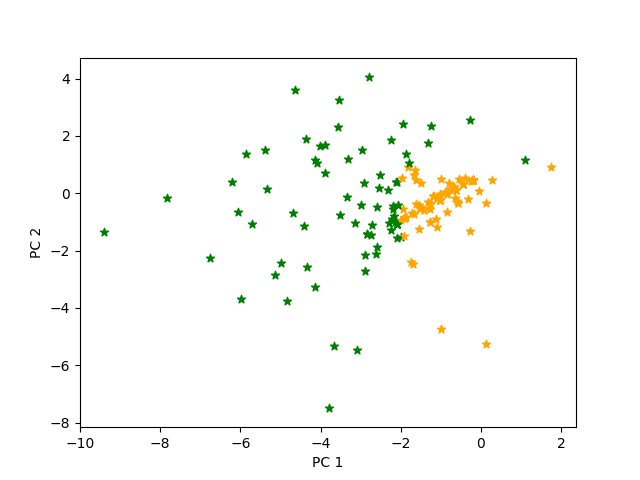
\includegraphics[scale=0.5]{../images/clusters_error_Depth_.png} \\ 
		
		Green is benign data and yellow is malignant. As it was stated before, all three functions do a very similar job that's why results are so similar. Although clusters with Misclassification error seem to be somewhat more packed. \\
		Comparing to results on original data, training first 6 PCs components gives us 0.9824 accuracy on testing data. Pretty impressive. \\
		
	\end{enumerate}
	
	{\bf \item Conclusions.}\\
	 
	 Overall, in this project, we looked at two different ways to classify data: using k-nearest neighbors algorithm and using classification decision trees. kNN was much easier to implement and it ran a little bit faster than decision trees algorithm. I also received better classification accuracy with kNN algorithm. Decision Trees Algorithm was not as trivial as it looked. It also ran much longer than kNN, because we had to do so many comparisons  before we could decide how to split our nodes. Also I received lower accuracy on my tests classification with using decision trees, although using PCA for data dimensionality reduction made classification accuracy results higher a bit higher. In general, both algorithms worked well for classifying given data. 
\end{enumerate}
	
	
	
	
	
	
	
\end{document} 